\documentclass{report}
\usepackage[pdftex]{graphicx}


\begin{document}


\begin{titlepage}

\vspace*{\fill}
\begin{center}
testingTemperature Monitoring System \hspace*{\fill}
by Mike Guzior, Jason Pearson \hspace*{\fill}
Marcel Englmaier and Justin Koehler \hspace*{\fill}
3/16/2014 \hspace*{\fill}
Client: John Kapenga \hspace*{\fill}
Advisor: John Kapenga \hspace*{\fill}
\end{center}
\vspace*{\fill}
\end{titlepage}
\newpage
\tableofcontents
\newpage

\subsection*{Abstract}
\addcontentsline{toc}{subsection}{Abstract}
The goal of this project is to create an easy to use and low cost temperature monitoring system for anyone to use. The web end will allow the user to login in and view room statistics, as well as set warnings on thresholds. With the thresholds we would allow the user to select actions based on the threshold such as sending a text when it reaches a certain temperature.  The room will contain a Raspberry Pi equipped with sensors which will use Ethernet to communicate to the web end and update information. The reason for using the Raspberry Pi’s is that we would be able to create a low cost sensor and be able to customize the code on the Pi as well. 
\newpage
\subsection*{Background}
\addcontentsline{toc}{subsection}{Background}
	Western Michigan currently uses the Temperature @lert WiFi Edition to keep track of the temperature of rooms around campus. These sensors work very well but their major flaw is that they are very expensive. These sensors cost upwards of two hundred dollars per sensor and have many features that are neat, but unnecessary for our purposes. To alleviate this problem we proposed to create a server that would communicate with a network of home brewed sensor computers. The server was created by another Western Michigan Computer Science senior design team and it currently is used to communicate with the @lert sensors.  
	\newline
	\indent
	The currently used Temperature @lert WiFi sensor has accuracy of \pm.$5\,^{\circ}{\rm C}$. The max and minimum temperatures that the current sensor will calculate are -$10\,^{\circ}{\rm C}$ and +$85\,^{\circ}{\rm C}$. The current sensor also gives humidity readings. This is not high priority, but if we are able to implement it that would be desirable. The humidity readings that the current sensors give are between 10\% and 90\% relative humidity. This relative humidity has \pm3\% relative humidity accuracy One major feature of the sensor is the fact that it can be used over the network using wired or wireless connections. The wireless specs that it abides by are the 802.11b/g standards and allow for WPA/WEP security. These are the features that are used by the system that we need to implement on our client devices.
	\newline
	\indent
	TODO: talk about the other features that the device has and how similar features only need to be implemented on the server side.
	\newline
	\indent
\newpage

	
\subsection*{Design Decisions}
\addcontentsline{toc}{subsection}{Design Decisions}
Raspberry Pi: We decided to use the to connect to the temperature and humidity sensor because it is cost efficient and is able to send and receive data from the monitoring server. Other alternatives we looked at are the Arduino and the MSP430, but we ended up deciding on the raspberry pi because there was more documentation and had all the required hardware in one bundle.. Also Raspberry Pi’s require less hardware configuration allowing a end user with less hardware skills to still be able to utilize our project.
Git: Team members were more familiar with the workings of Git and could be used with a GUI.
Sensor: Team members spent a considerable amount of time exploring possible sensors, with the requirements being that the final solution utilize temperature and humidity sensing. As a single package, multiple solutions were found, but are currently too expensive to make them feasible. Much research was done into finding ones with Dallas One-Wire capability. One-Wire is a protocol which identifies each device separately, and can query each device using a single wire. Currently, only the DS18B20 temperature sensor is being used. A fitting humidity sensor for less that 5 dollars has not been found yet, but is still being looked for.
We have also decided to separate the project into 4 main functional pieces which each need their required spikes. The flow of the normal communication is as displayed as below.
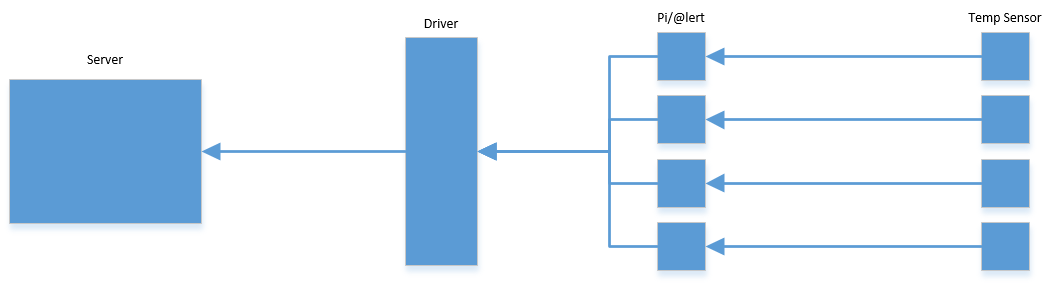
\includegraphics{DataFlowFlowChart.PNG}
\newpage
\subsection*{Stories -- Requirements}
\addcontentsline{toc}{subsection}{Stories -- Requirements}
	This project requires a server running linux, we will be using Ubuntu on this system. We also require a temperature sensor of your choice. We will be interfacing with the Temperature @lert WiFi edition TM-WIFI220 as well as Raspberry Pi’s running rasberian. If you would like WiFi connectivity for your Raspberry Pi like we are going to, we will use a wireless receiver.
	TODO: List the parts that we are going to use for the wireless reciever and the other parts

\newpage
\subsection*{Stories -- Functional}
\addcontentsline{toc}{subsection}{Stories -- Functional}
Use a temperature sensor to monitor the temperature of the servers room located on the CEAS campus.
Check the humidity of the server rooms located on the CEAS campus.
Send the data to a server to be checked.
Use timers to make sure that communication with the servers are not lost
Send text messages and emails to the server administrators to alert them of loss of server connection and temperatures that are higher than the recommended level.
Establish permissions for the various admins that will be monitoring the system.

\newpage
\subsection*{Spikes}
\addcontentsline{toc}{subsection}{Spikes}
	To do these stories we will be creating spikes to show that critical sections are actually plausible. After we do this we combine the spikes and add minor code to complete the system. Some of our spikes are raspberry pi temperature retrieval code, raspberry to server communications, and sending emails to admins to name a few. 
\newpage
\subsection*{Resources}
\addcontentsline{toc}{subsection}{Resources}
Raspberry Pi
Temperature Sensors
Humidity Sensors
Web Server
Soldering Equipment
Operating System loaded SD Cards with Rasperian
Power connectors for Raspberry pi
WiFi Connectors for Raspberry pi
\newpage
\subsection*{Feasibility}
\addcontentsline{toc}{subsection}{Feasibility}
Feasibility
	Based the cost of the hardware and the previous source code the feasibility of this project is high with many of the features being of low to mid risk. Extra features can be implemented very easily for future releases.
References
	For everything raspberry pi we use these sites
http://www.raspberrypi.org/
http://www.raspbian.org/
C Programming 2nd Edition
For everything web server these are the sites we use
	http://laravel.com/docs/quick
http://www.w3schools.com/
\newpage
\subsection*{Glossary}
\addcontentsline{toc}{subsection}{Glossary}
\begin{description}
\item [GUI] \hfill \\
Graphical User Interface. The windows a user interacts with.
\item [MSP430] \hfill \\
A 16-bit microcontroller platform made by Texas Instruments.
\item [Raspberry Pi] \hfill \\
 A credit-card-sized single-board computer developed by the Raspberry Pi Foundation.
\item [Arduino] \hfill \\
A series of microcontrollers that are very commonly used for computer to real world communications.
\item [Rasberian] \hfill \\
 A Debian based operating system that we will use for our Raspberry Pi’s
\item [CEAS] \hfill \\
College of Engineering and Applied Sciences at Western Michigan University.
\end{description}
\newpage
\subsection*{Ownership}
\addcontentsline{toc}{subsection}{OwnerShip}
	Our project will be under the GNU license and will be open source and will be hosted for all to access and modify as they desire on github.

\end{document}
